%%%%%%%%%%%%%%%%%%%%%%%%%%%%%%%%%%%%%%%%%%%%%%%%%%%%%%%%%%%%%%%%%
%  _____       ______   ____									%
% |_   _|     |  ____|/ ____|  Institute of Embedded Systems	%
%   | |  _ __ | |__  | (___    Wireless Group					%
%   | | | '_ \|  __|  \___ \   Zuercher Hochschule Winterthur	%
%  _| |_| | | | |____ ____) |  (University of Applied Sciences)	%
% |_____|_| |_|______|_____/   8401 Winterthur, Switzerland		%
%																%
%%%%%%%%%%%%%%%%%%%%%%%%%%%%%%%%%%%%%%%%%%%%%%%%%%%%%%%%%%%%%%%%%


\pagenumbering{Roman}

\appendix



\chapter{Offizielle Aufgabenstellung}\label{chap.anhang_aufgabenstellung}
\section*{Beschreibung der Projektarbeit Pa15\_gelk\_1}\label{sect.aufgabenstellung}

In dieser Projektarbeit sollen Versuche entwickelt werden, die für das Modul DTP2 verwendet werden können. Die Arbeit besteht aus zwei Teilen: \\
\newline
Im ersten Teil der Arbeit sollen Versuche entwickelt werden, mit denen folgende Timing Artifakte demonstriert werden können. Dies soll zum zu einem vertieften Verständnis der digitalen Design Grundlagen führen.
\newline
\begin{itemize}
	\item Erzeugung von Glitches mit einem Zähler und nachgeschaltetem Dekoder. Sichtbarmachung der Glitches mit einem Oszilloskop. Betätigen des asynchronen Resets vom Decoder aus. 

	\item Provozieren und sichtbarmachung von Metastabilen Zuständen. Hierfür kann z.B. eine Schaltung mit zwei asynchronen externen Takten aufgebaut werden. 
\end{itemize}
\bigskip
Im zweiten Teil soll mit dem dem Direct Digital Synthesis Verfahren ein Synthesizer mit vielfältigen Klangfarben entwickelt werden. Damit kann anspruchsvolle digitale Schaltungstechnik umgesetzt werden. Zum erreichen der Klangvielfalt können mehrere DDS Generatoren gleichzeitig, mit unterschiedlichen Frequenzen und Phasen betrieben werden. Möglich ist auch eine Frequenzmodulation mit einem zweiten Generator oder Ändern des Volumens mit einer Hüllkurve. Die Ansteuerung soll mit Hilfe eines MIDI Interfaces, welches Polyphonie (mehrere Klaviertasten gleichzeitig gedrückt) unterstützt. Die Implementierung soll im FPGA erfolgen. In der Implementierungsphase der Arbeit soll das Timing der FPGA Implementierung genau betrachtet werden.
\\[0.1cm]
Am Ende soll eine Referenzimplementierung in Anlehnung an den Yamaha DX7 für das Modul DTP2 entstehen 



\chapter{Aufgabenspezifikation für den zweiten Teil}\label{chap.anhang_aufgabenstellung_neu}

\begin{itemize}
\item Midi Interface for Keyboard für Polyphonie nach Konzept von gelk\\
o   10 Frequenz Control Ausgänge zur Steuerung der Tonhöhe des Generators\\
o   10 On/Off Ausgänge Ton on/off\\
o   UART wird geliefert von gelk\\
o   VHDL wird von Grund auf neu erstellt.
\item 10 DDS implementieren und mit Mischer Mischen
\item Script basierte Testbench. Testbench erzeugt serielle Midi Dtaen, so wie sie auf dem DIN Stecker vorkommen (logisch)
\item Testbench liest eine Testscript Datei ein, in welcher die Tastendrücke eines Keyboards abgebildet werden können. Midi Poliphony Spec muss durch die Testbench unterstützt werden können. Velocity muss nicht unterstützt werden.
\item FM Modulation – Tetstbench im Matlab
\item Kein VHDL code ohne Testbench.
\item Block level testbench. Unit Tests.
\end{itemize}  

Abgrenzung:
\begin{itemize}
\item Keine Hüllkurve
\item Keine Ausgabe der Velocity aud Midi controller
\item Kein Bluetotth
\end{itemize} 
Zeitplan:
\begin{itemize}
\item 2.5 Wochen Midi Controller incl. 10 DDS
\item 2.5 Wochen FM Synthese 
\end{itemize} 

Unterstützung:
\begin{itemize}
\item Midi Controller/gelk
\item FM-Synthese/rosn
\end{itemize} 

Falls Midi nicht zum geplanten Zeitpunkt fertig wird, wird FM-zurückgestellt. Alle oben genannten Punkte sind Pflicht.
Nicht Fertigstellung hat Einfluss auf die Benotung.




\chapter{Konzept Keyboard Dekoder}\label{chap.anhang_hans_midicontrol}
\begin{figure}[H]
	\centering
	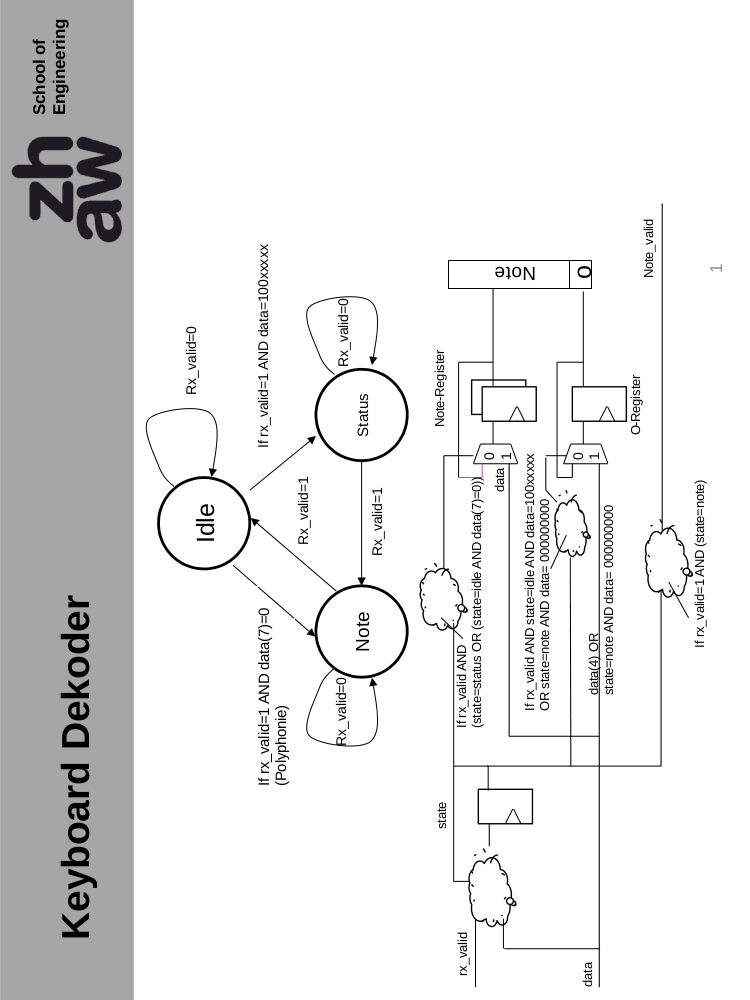
\includegraphics[width=0.9\textwidth]{images/midi_interface/Midi_Konzept_midi_control.png}
	\caption{Midi Controller Spezifikation}
	\label{fig.Hans_midicontrol}
\end{figure}





\chapter{Konzept Polyphonie}\label{chap.anhang_hans_polyphonie}
\begin{figure}[H]
	\centering
	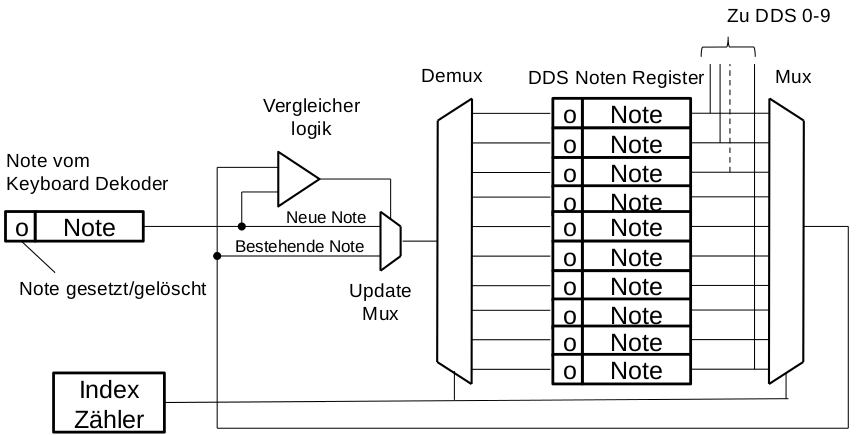
\includegraphics[width=0.9\textwidth]{images/midi_interface/Konzept_Hans_polyphonie.png}
	\caption{Spezifikation Polyphonie-Block}
	\label{fig.Hans_polyphonie}
\end{figure}



\chapter{CD mit Projektdateien}\label{sect.anhang_cd}


\chapter{Top Synthesizer}\label{chap.anhang_top_synthesizer}

In die bestehenden Blöcke und Signale wird das MIDI Interface wiefolgt eingebaut:\\
\begin{figure}[H]
	\centering
	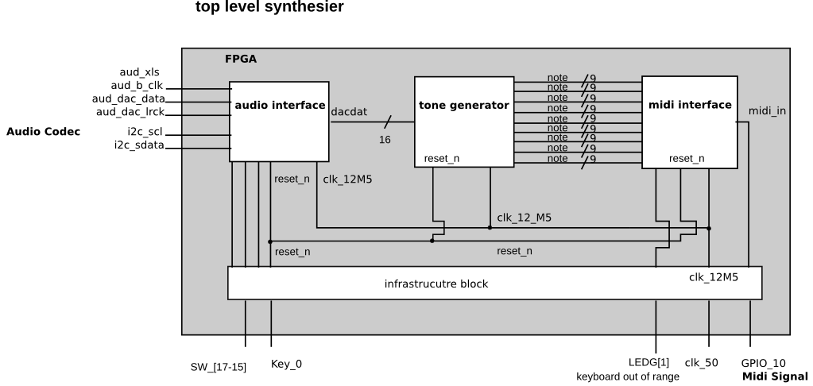
\includegraphics[width=0.9\textwidth]{images/midi_interface/top_synthesizer_block_saled.png}
	\caption{Top Synthesizer mit MIDI Interface: Blockschaltbild}
	\label{fig.top_synthesizer_block}
\end{figure}

Hier ist das Konzept der Umsetzung des MIDI Interface detaillierter beschrieben:\\
\begin{figure}[H]
	\centering
	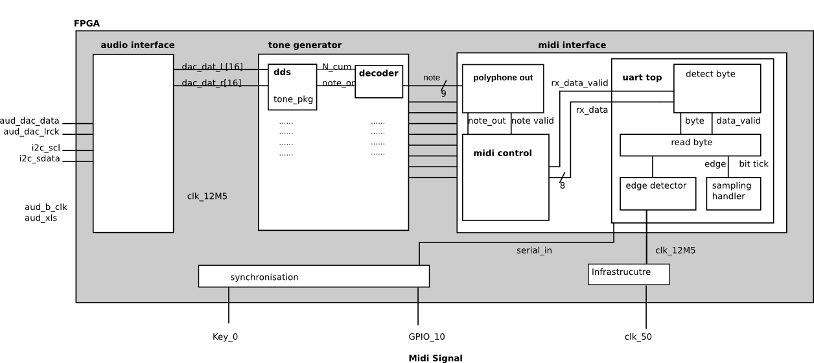
\includegraphics[width=0.9\textwidth]{images/midi_interface/top_synthesizer_detail_scaled.png}
	\caption{Top Synthesizer mit MIDI Interface: Detailansicht}
	\label{fig.top_synthesizer_detail}
\end{figure}



